main.texには8つのセクションとそれに対応するサブファイルの取り込みが書かれている。
対応するそれぞれのサブファイルは生成された直後は空のファイルである。
そのサブファイルの編集が文書作成の主要な作業になり、作成にかかる時間の大部分がそれに当てられる。

最初のセクションとサブファイルは、それぞれ「インストール」と「installation.tex」である。
おそらく、セクションの一部を編集した段階で、pdfファイルがどのように出来ているかを見るためにテスト・コンパイルすることがあるだろう。
多くの場合、編集とテスト・コンパイルの間を何回も行ったり来たりするものである。

もしも、文書がさほど大きくないならば、rakeを用いるのがテスト・コンパイルには最も良い。
というのは、さほどコンパイル時間もかからず、文書全体のpdfを見ることができるからである。
このチュートリアルは、どちらかといえば小さい文書であるから、rakeをテスト・コンパイルに用いるのが良い。
\begin{verbatim}
\subsection{動作条件}
Buildtoolsには次のものが必要である。
\begin{enumerate}
\item Linux OS とbash
\item LaTeXシステム
\item MakeまたはRake
\end{enumerate}
 ... ...
 ... ...
\end{verbatim}
編集が終わったら(もちろん、チュートリアルであるから、ソースファイルのinstallation.texをコピーしても何ら差し支えない)、下記のようにタイプしてpdfを見てみよう。
\begin{verbatim}
$ rake
$ evince チュートリアル.pdf
\end{verbatim}

\begin{center}
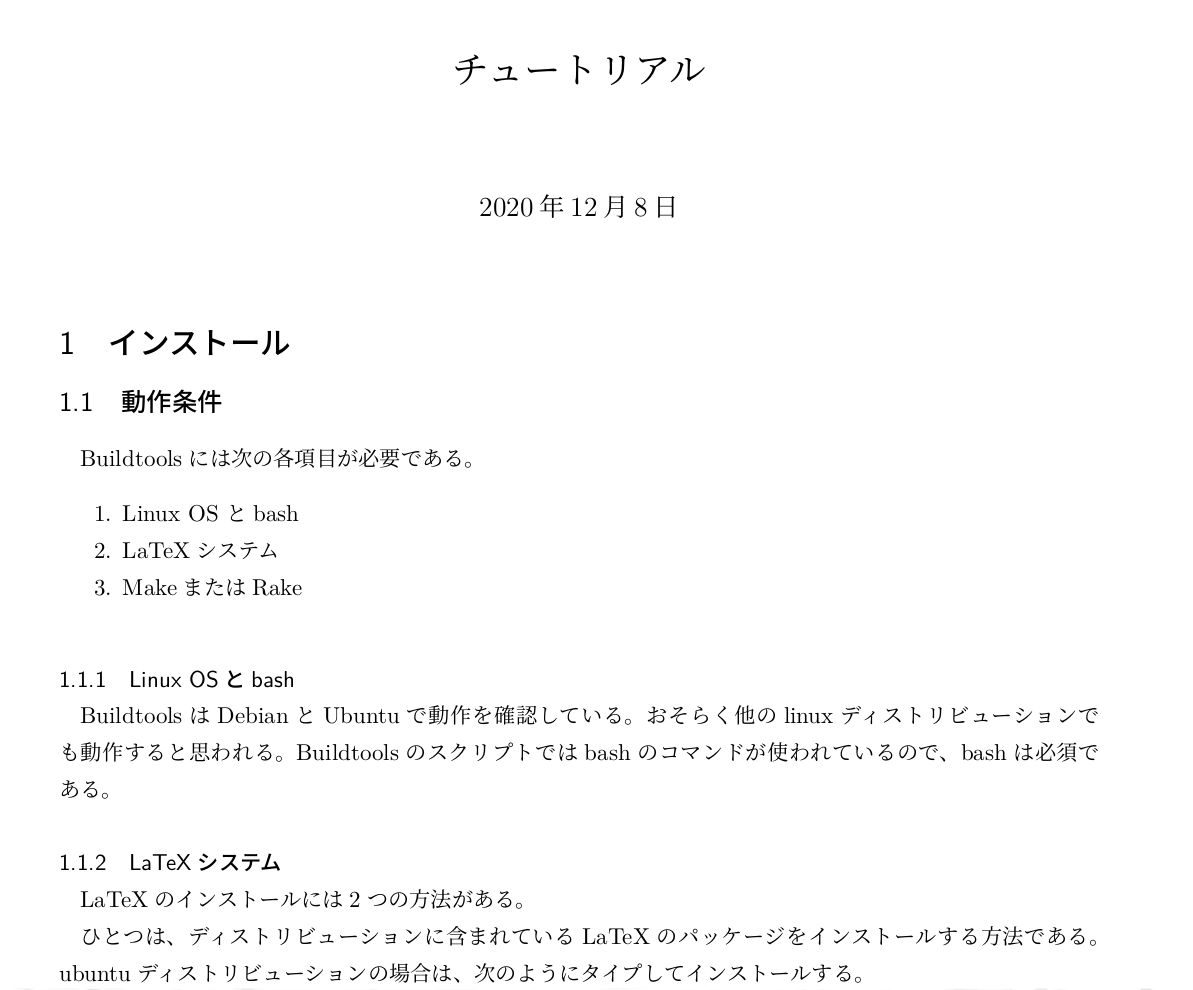
\includegraphics[width=12cm]{Tutorial_2.png}
\end{center}
